\documentclass[a4paper,12pt]{article}
\usepackage[spanish]{babel}
%graficos
\usepackage{graphicx}
\graphicspath{{../resultados_analisis_eolico/graficos/}}
\usepackage{float}
\setlength{\parindent}{0pt}
\usepackage{parskip}
\usepackage{amsmath}
%margenes
\usepackage{geometry}
\newgeometry{bottom=2.5cm, top=2.5cm, left=3cm, right=3cm}
\usepackage{amssymb}
\usepackage{xcolor} % para colores bonitos en el código
%Encabezado
\usepackage{fancyhdr}
\usepackage{titling}
\pagestyle{fancy}
\lhead[]{\thetitle}
\chead[]{}
\rhead[]{}
%opening
\title{\textbf{Análisis Técnico del Potencial Eólico en Santa Cruz, Bolivia}}
\author{Rodrigo Andres Valda Alcoba}
\date{\today}

\begin{document}
	
	\maketitle
	\begin{abstract}
			Este estudio presenta un análisis técnico del recurso eólico en el departamento de Santa Cruz, Bolivia, basado en datos horarios del año 2024 obtenidos del conjunto de reanálisis ERA5. Se procesaron un total de 491\,904 registros utilizando herramientas computacionales en Python, con el objetivo de evaluar la viabilidad del aprovechamiento del viento como fuente de energía renovable.
			
			Los resultados indican una velocidad media anual del viento de 2.91 m/s, una mediana de 2.56 m/s y una desviación estándar de 1.73 m/s. El ajuste a la distribución de Weibull arrojó parámetros \(c = 3.15\) y \(k = 1.75\), lo que describe una distribución ligeramente asimétrica y concentrada en velocidades bajas. La densidad media de potencia eólica fue estimada en 15 W/m² y el factor de capacidad resultó ser aproximadamente 3.0\%, lo que se traduce en una generación anual estimada de 1.27 GWh para un aerogenerador con rotor de 100 m de diámetro.
			
			Estos valores reflejan un recurso eólico limitado, clasificado como pobre según estándares internacionales, aunque suficiente para fines demostrativos en el contexto de análisis de datos y modelado energético.
		\end{abstract}
	
	\section{Introducción}
		El uso de fuentes de energía renovable se ha convertido en un pilar clave para impulsar un desarrollo sostenible en las sociedades actuales. Entre estas alternativas, la energía eólica sobresale por su capacidad de generar electricidad de manera limpia, abundante y con un impacto ambiental reducido. No obstante, antes de considerar la implementación de proyectos eólicos en una zona específica, es indispensable llevar a cabo un análisis técnico riguroso que permita evaluar tanto su viabilidad como su verdadero potencial energético.
		
		En este sentido, la presente investigación se enfoca en el departamento de Santa Cruz, Bolivia, una región cuyas condiciones geográficas y climáticas podrían resultar favorables para el aprovechamiento de la energía del viento. A pesar de su importancia estratégica para el desarrollo energético del país, el potencial eólico de esta área ha sido poco explorado con el apoyo de herramientas modernas de análisis de datos y simulación computacional.
		
		El propósito de este trabajo es utilizar técnicas de procesamiento y visualización de datos meteorológicos obtenidos del reanálisis ERA5, empleando herramientas desarrolladas en Python. Esto permitirá estimar la distribución de velocidades del viento, analizar su comportamiento a lo largo de las estaciones y durante el día, así como calcular la posible generación de energía eléctrica. Los resultados no sólo buscan describir las características del recurso eólico disponible, sino también ofrecer una base técnica sólida para futuras investigaciones o proyectos en este ámbito.
		
		Con este artículo, se invita al lector a conocer de manera detallada la metodología aplicada, los hallazgos obtenidos y sus posibles implicaciones en el contexto energético regional, con el fin de aportar a una valoración realista y fundamentada de las energías renovables en Bolivia.
		
	\section{Objetivos}
		\subsection{Objetivos Generales}
			\begin{itemize}
				\item Analizar el comportamiento del recurso eólico en la región de Santa Cruz, Bolivia, mediante el procesamiento y visualización de datos meteorológicos, con el fin de demostrar técnicas de análisis y modelado aplicadas a potenciales fuentes de energía renovable.
			\end{itemize}
		\subsection{Objetivos Especificos}
			\begin{itemize}
				\item Recolectar y procesar datos climáticos y meteorológicos relevantes para la evaluación del viento en la zona de estudio, utilizando archivos ERA5 en formato ".grib".
				\item Desarrollar y aplicar métodos computacionales para decodificar, analizar y visualizar la velocidad y dirección del viento en Santa Cruz.
				\item Realizar simulaciones y ajustes estadísticos, como la distribución de Weibull, para caracterizar la variabilidad y el comportamiento del viento en diferentes periodos.
				\item Generar mapas, gráficos y rosas de viento que permitan visualizar patrones y tendencias del recurso eólico en la región.
				\item Evaluar el potencial energético a partir de los datos analizados, estimando la producción posible de energía eólica en distintos escenarios.
			\end{itemize}
	\section{Metodología}
		\subsection{Fuente de Datos}
		
			En este estudio se emplearon datos del conjunto de reanálisis ERA5, elaborado por el Centro Europeo de Pronósticos Meteorológicos a Mediano Plazo (ECMWF). Este conjunto de datos representa la quinta generación de productos de reanálisis climático a nivel global y ofrece estimaciones detalladas de distintas variables atmosféricas desde 1940 hasta la actualidad, con mejoras notables respecto a su versión anterior, ERA-Interim.
			
			Para el desarrollo de este trabajo se descargó la serie completa de datos horarios correspondientes a todo el año 2024, sin excluir ningún día, mes ni hora, abarcando toda la extensión territorial de Bolivia. Las variables seleccionadas fueron las componentes zonal (u) y meridional (v) del viento a 10 metros de altura, con una resolución espacial de 0.25° x 0.25°. Estas variables resultan clave para calcular tanto la velocidad como la dirección del viento, parámetros esenciales en la evaluación del potencial eólico en el territorio boliviano.
			
		\subsection{Procesamiento de Datos}
			
			Para analizar el potencial del viento en Santa Cruz, se trabajó con archivos de datos en formato GRIB proporcionados por ERA5, utilizando las librerías xarray y cfgrib. El primer paso fue abrir el archivo que contenía la información del viento, en particular las componentes zonal (u10) y meridional (v10), ambas medidas a una altura de 10 metros.
			
			A partir de estas componentes, se calcularon dos variables clave para el estudio: por un lado, la velocidad del viento, obtenida mediante la raíz cuadrada de la suma de los cuadrados de u y v; y por otro, la dirección del viento, que se determinó usando la función arcotangente, ajustando el resultado para expresarlo en grados dentro del rango de 0 a 360°.
			
			Después, se aplicó un filtro espacial para extraer exclusivamente los datos que correspondían a la zona geográfica de Santa Cruz, Bolivia, definiendo un rango específico de latitudes y longitudes. Una vez extraída esta información, se transformó en un formato tabular utilizando un DataFrame de Pandas, y se exportó a un archivo CSV para facilitar su análisis y visualización.
			
			Gracias a este procedimiento, se logró generar una base de datos clara y bien estructurada con registros horarios de velocidad y dirección del viento a lo largo de todo el año 2024, específicamente para la región de interés.
			
		\subsection{Análisis Estadístico del Viento}
		\label{subsec:estadistico}
		
		Para entender el comportamiento del viento en la región, se aplicaron diversas técnicas estadísticas, entre ellas:
		
		\begin{itemize}
			\item \textbf{Distribución de Weibull}: Se ajustó esta distribución de probabilidad mediante mínimos cuadrados, utilizando la función \texttt{curve\_fit} de SciPy. La función de densidad utilizada fue:
			\begin{equation}
				f(v,c,k) = \frac{k}{c} \left( \frac{v}{c} \right)^{k-1} e^{-(v/c)^k}
				\label{eq:weibull}
			\end{equation}
			donde \(v\) representa la velocidad del viento, \(c\) es el parámetro de escala (asociado a la velocidad promedio) y \(k\) el parámetro de forma (que refleja la variabilidad del viento).
			
			\item \textbf{Estadísticas descriptivas}: Se calcularon métricas que resumen el comportamiento general del viento:
			\begin{itemize}
				\item Velocidad media: \(\bar{v} = \frac{1}{n}\sum_{i=1}^{n} v_i\)
				\item Mediana: valor central del conjunto de velocidades ordenadas
				\item Desviación estándar: \(\sigma = \sqrt{\frac{1}{n}\sum_{i=1}^{n} (v_i - \bar{v})^2}\)
				\item Percentiles: 5\%, 25\%, 75\% y 95\%
			\end{itemize}
			
			\item \textbf{Variabilidad temporal}: Se analizó cómo cambia la velocidad del viento a lo largo del tiempo, considerando diferentes escalas:
			\begin{itemize}
				\item Variación mensual: promedio de velocidad por mes
				\item Variación horaria: velocidad promedio por hora del día
				\item Estacionalidad: comparación entre distintas épocas del año
			\end{itemize}
		\end{itemize}
		
		\subsection{Visualización de Datos}
		\label{subsec:visualizacion}
		
		Para facilitar la comprensión del comportamiento del viento, se generaron diversas visualizaciones:
		
		\begin{itemize}
			\item \textbf{Histograma de velocidades}: Muestra la frecuencia de ocurrencia de distintas velocidades, acompañado del ajuste de la distribución de Weibull.
			\item \textbf{Rosa de los vientos}: Diagrama polar que representa la dirección del viento, segmentado por rangos de velocidad (Figura %\ref{fig:rosa}).
			\item \textbf{Variación temporal}: Conjunto de gráficos que incluyen:
			\begin{itemize}
				\item Serie de tiempo de velocidades
				\item Barras con promedios mensuales
				\item Línea de variación horaria diaria
				\item Diagramas de caja por mes
			\end{itemize}
			\item \textbf{Mapas geoespaciales}:
			\begin{itemize}
				\item Mapa estático de la distribución espacial de velocidades
				\item Mapa interactivo que muestra el potencial eólico (Figura %\ref{fig:mapa})
			\end{itemize}
			\item \textbf{Panel estadístico}: Visualización combinada con histograma, diagrama de caja, curva de percentiles y función de distribución acumulativa.
		\end{itemize}
		
		\subsection{Estimación del Potencial Eólico}
		\label{subsec:potencial}
		
		Para estimar el potencial energético del viento en la región, se emplearon los siguientes métodos:
		
		\begin{itemize}
			\item \textbf{Modelo de curva de potencia}: Se utilizó un modelo simplificado de aerogenerador con las siguientes condiciones:
			\begin{equation}
				P(v) = 
				\begin{cases} 
					0 & v < 3 \\
					\frac{1}{2} \rho A v^3 C_p & 3 \leq v < 12 \\
					P_{\text{nominal}} & 12 \leq v < 25 \\
					0 & v \geq 25
				\end{cases}
				\label{eq:potencia}
			\end{equation}
			donde \(\rho = 1.225  \text{kg/m}^3\) es la densidad del aire, \(A\) es el área del rotor (\(A = \pi (D/2)^2\) con \(D = 100  \text{m}\)) y \(C_p = 0.59\) es el coeficiente de potencia.
			
			\item \textbf{Indicadores de desempeño}:
			\begin{itemize}
				\item Factor de capacidad: \(\text{FC} = \frac{\text{Energía real generada}}{\text{Energía máxima posible}} \times 100\%\)
				\item Horas equivalentes a potencia nominal: \(h_{\text{eq}} = \frac{\text{Energía anual}}{P_{\text{nominal}}}\)
				\item Densidad de potencia eólica: \(P_d = \frac{1}{2} \rho v^3\)
			\end{itemize}
			
			\item \textbf{Análisis de viabilidad}:
			\begin{itemize}
				\item Clasificación del recurso según velocidad media
				\item Porcentaje de velocidades útiles (entre 3 y 25 m/s)
				\item Evaluación de estacionalidad
				\item Estimación de la energía generada anualmente
			\end{itemize}
			
			\item \textbf{Reporte técnico}: Se generó automáticamente un informe con:
			\begin{itemize}
				\item Principales estadísticas del recurso
				\item Clasificación del viento en la zona
				\item Estimaciones de producción energética
				\item Recomendaciones técnicas para su aprovechamiento
			\end{itemize}
		\end{itemize}
		\subsection{Herramientas Computacionales}
		
		El análisis y procesamiento de los datos se llevó a cabo utilizando Python 3, apoyado en un conjunto de librerías especializadas que facilitaron el manejo, análisis estadístico y visualización de información científica. Entre las principales herramientas utilizadas se encuentran:
		
		\begin{itemize}
			\item \texttt{os} y \texttt{math}, para operaciones básicas del sistema y funciones matemáticas.
			\item \texttt{numpy}, para cálculos numéricos y manejo de arreglos multidimensionales.
			\item \texttt{pandas}, para manipulación y análisis de datos en estructuras tabulares.
			\item \texttt{matplotlib.pyplot} y \texttt{seaborn}, para la generación de gráficos estadísticos y visualizaciones.
			\item \texttt{scipy.optimize.curve\_fit}, utilizada para ajustar modelos estadísticos a los datos, como en el caso de la distribución de Weibull.
			\item \texttt{plotly.express} y \texttt{plotly.graph\_objects}, que permitieron la creación de gráficos interactivos y visualizaciones dinámicas.
			\item \texttt{xarray}, para la lectura y manipulación de archivos en formato GRIB del conjunto ERA5.
		\end{itemize}
		
		El uso de estas herramientas permitió contar con un entorno robusto y flexible para procesar grandes volúmenes de datos climáticos, facilitando tanto el análisis estadístico avanzado como la generación de visualizaciones detalladas sobre el comportamiento del recurso eólico en la región de Santa Cruz.
		
		Para el desarrollo del presente proyecto se utilizó la distribución Linux Ubuntu como sistema operativo, empleando como entorno de desarrollo integrado (IDE) PyCharm. Este entorno permitió una gestión eficiente e integrada del código, el análisis de datos y la visualización de resultados en un único espacio de trabajo, facilitando la interacción y el flujo de trabajo durante el proceso de investigación.
		
	\section{Resultados y Discusión}
	
	\subsection{Estadísticas Descriptivas del Viento}
	Se trabajó con 491\,904 registros horarios del año 2024 extraídos de ERA5. Las métricas calculadas son:
	\begin{itemize}
		\item Velocidad media anual: $\bar v = 2.91\ \mathrm{m/s}$
		\item Velocidad mediana: $2.56\ \mathrm{m/s}$
		\item Velocidad máxima registrada: $12.08\ \mathrm{m/s}$
		\item Velocidad mínima registrada: $0.01\ \mathrm{m/s}$
		\item Desviación estándar: $1.73\ \mathrm{m/s}$
		\item Coeficiente de variación: $59.6\%$
	\end{itemize}
	
	
	\begin{figure}[H]
		\centering
		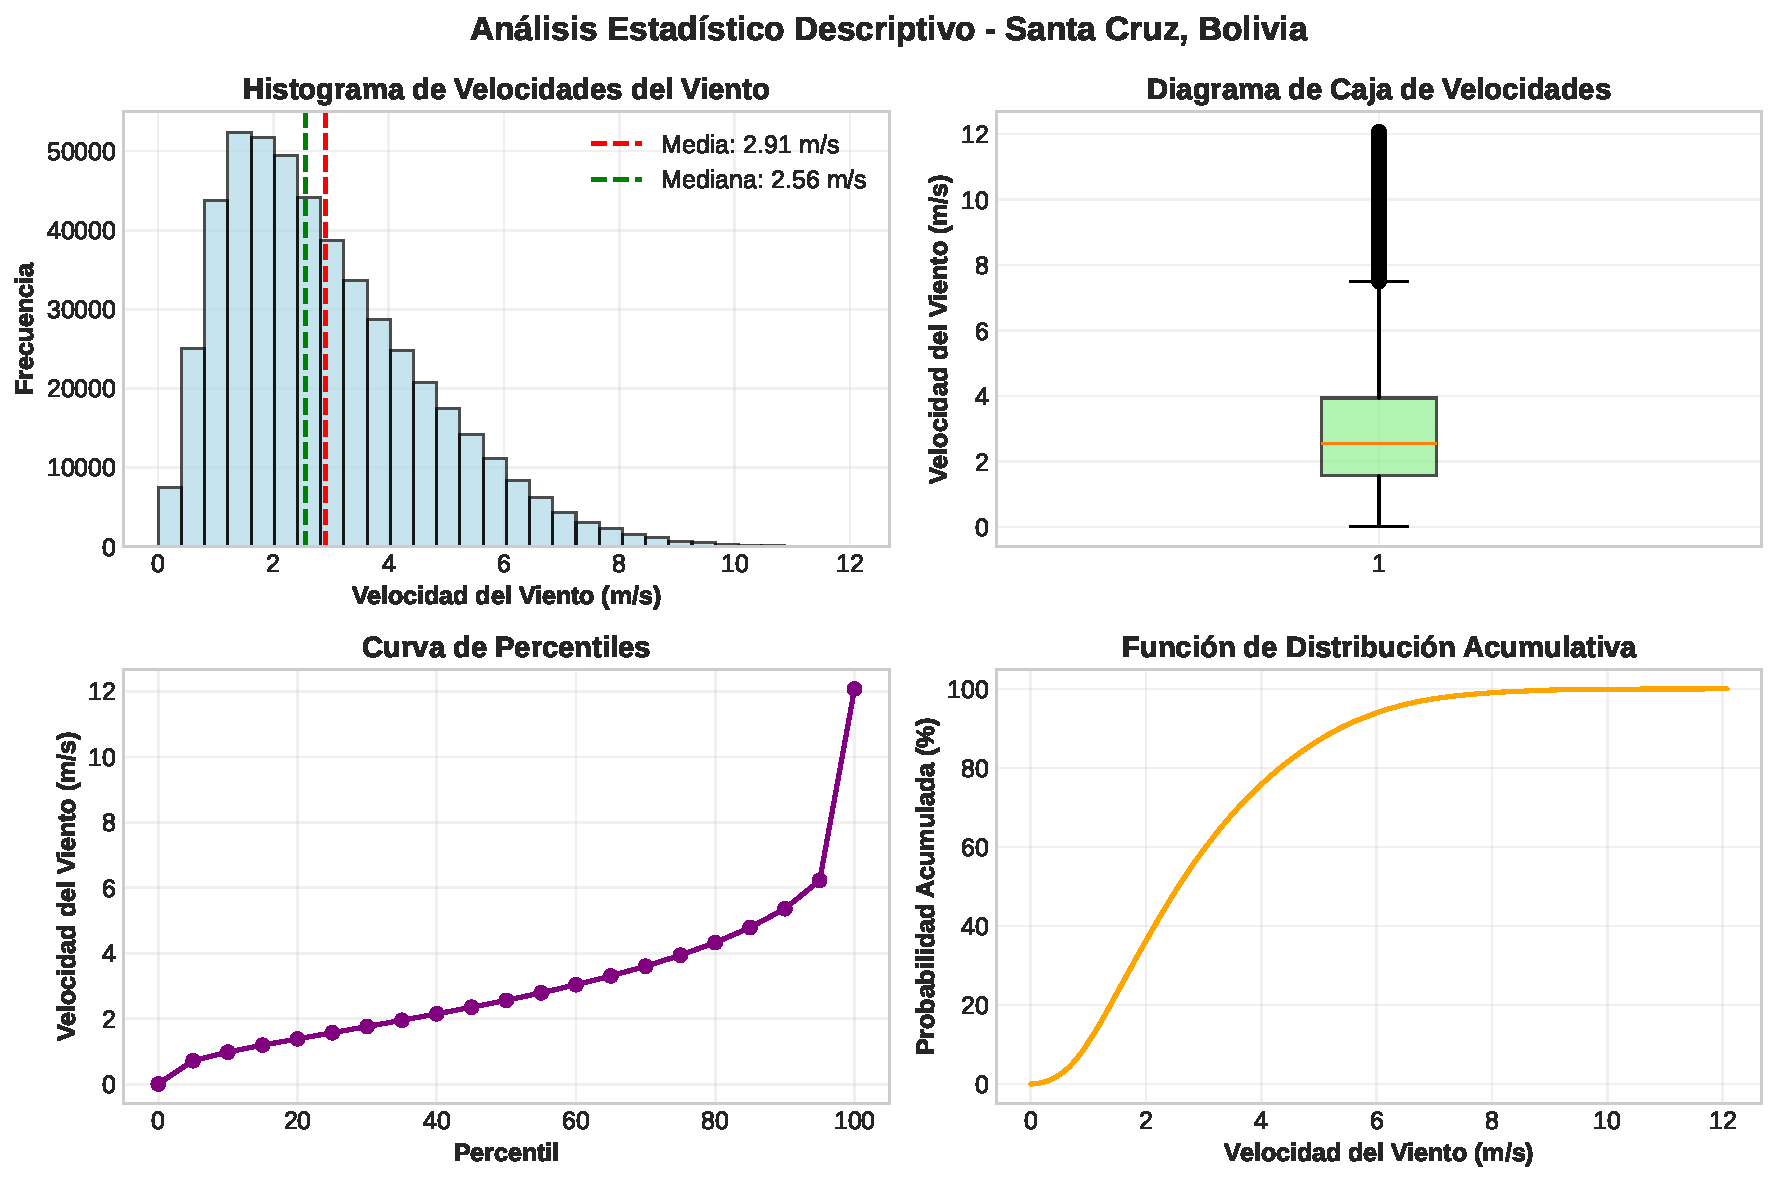
\includegraphics[width=1.0\textwidth]{estadisticas_descriptivas.pdf}
		\caption{Gráficas resultantes análisis estadistico descriptivo}
		\label{fig:estadistica}
	\end{figure}
	
	\subsection{Ajuste de Weibull}
	El ajuste mediante mínimos cuadrados a la distribución de Weibull
	\[
	f(v;c,k)=\frac{k}{c}\Bigl(\frac{v}{c}\Bigr)^{k-1}e^{-(v/c)^k}
	\]
	arrojó valores de $c=3.15\ \mathrm{m/s}$ y $k=1.75$. Este valor de $k>1$ sugiere una distribución unimodal con ligera asimetría, adecuada para describir el comportamiento del recurso eólico local.
	
		\begin{figure}[H]
			\centering
			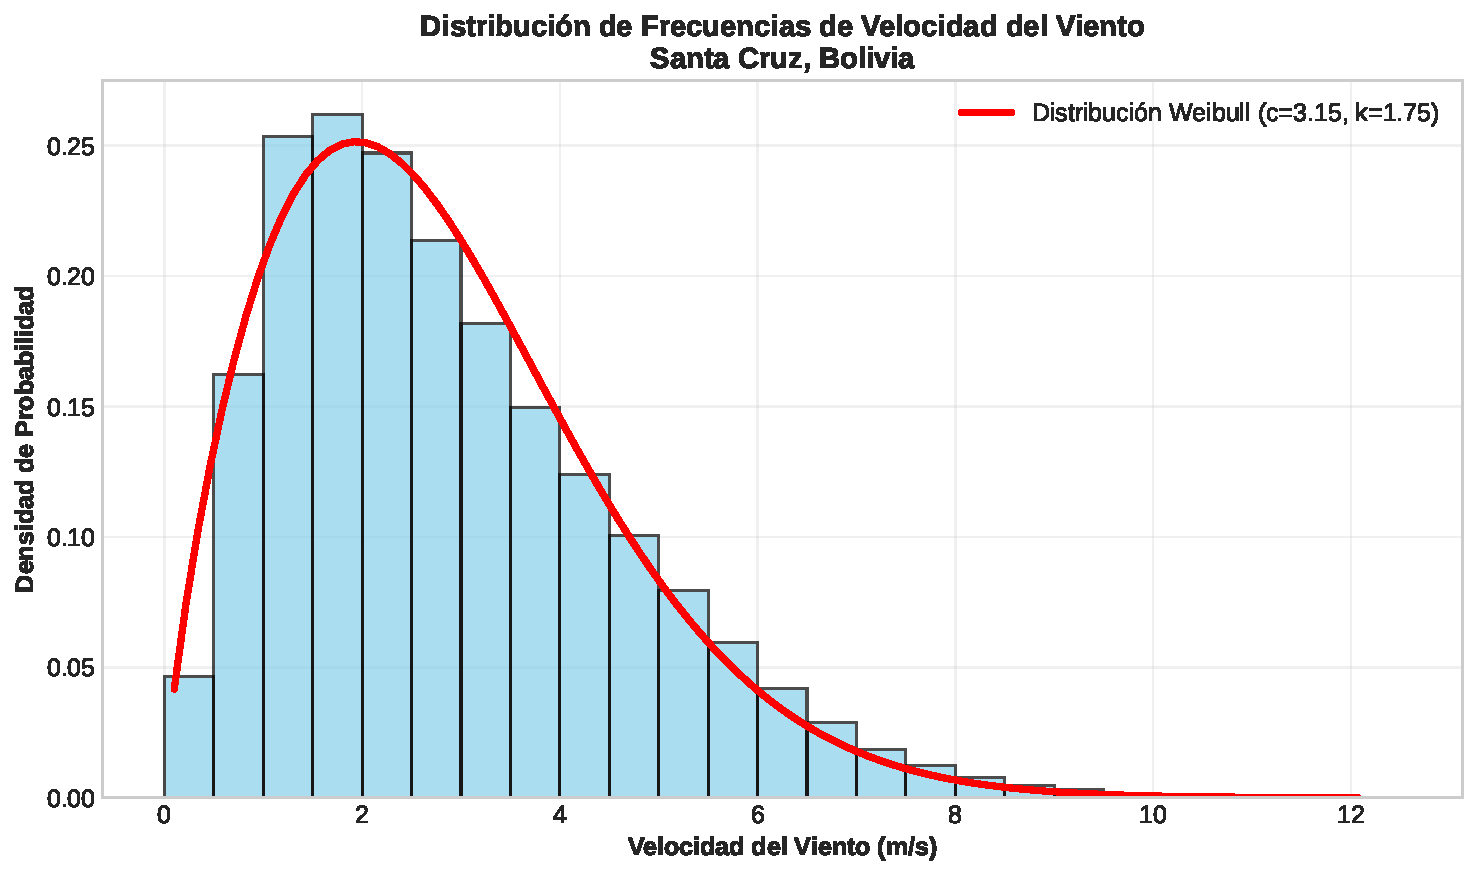
\includegraphics[width=0.7\linewidth]{histograma_velocidades}
			\caption{Distribución Weibull con c=3.15 y k=1.75}
			\label{fig:histogramavelocidades}
		\end{figure}
	\subsection{Clasificación del Recurso}
		Según la velocidad media anual, el recurso se clasifica como \textbf{POBRE} (<4.5 m/s), no viable económicamente, con densidad de potencia de $15\ \mathrm{W/m^2}$.
	\subsection{Variabilidad Temporal}
	
	\paragraph{Estacional}  
	Los promedios mensuales (Figura~\ref{fig:mensual}) revelan un máximo en junio ($3.47\ \mathrm{m/s}$) y un mínimo en febrero ($2.26\ \mathrm{m/s}$), con una amplitud total de $1.21\ \mathrm{m/s}$ entre estos extremos.
	
	\paragraph{Diurna}  
	El ciclo diario promedio (Figura~\ref{fig:diurno}) muestra picos de velocidad por la tarde y valores mínimos durante la noche. Sólo el 40.8\% de las horas supera el umbral de 3\,m/s necesario para generación eléctrica, lo que deja un 59.2\% de las horas sin producción aprovechable.
	
	\begin{figure}[H]
		\centering
		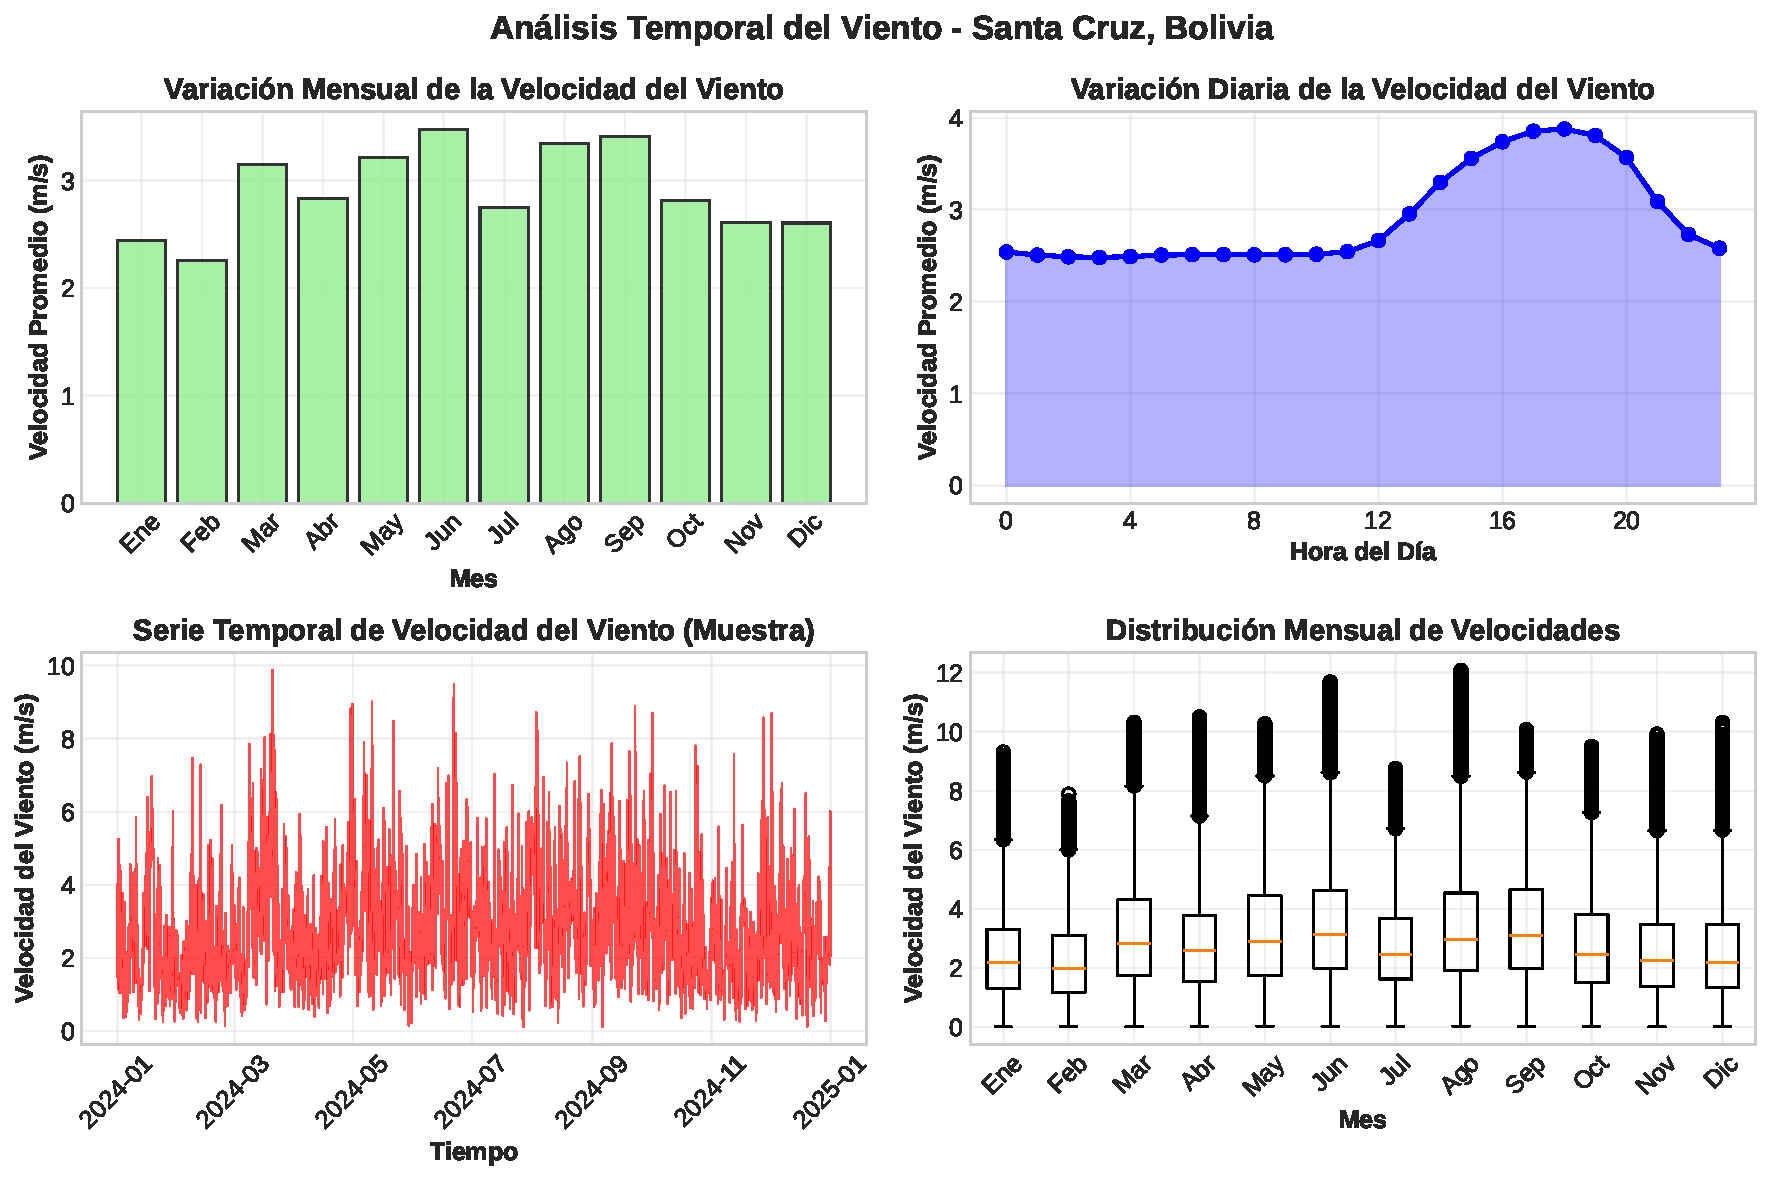
\includegraphics[width=1.0\textwidth]{variacion_temporal.pdf}
		\caption{Variación temporal de la velocidad del viento en Santa Cruz: promedio mensual y ciclo diario.}
		\label{fig:mensual}
		\label{fig:diurno}
	\end{figure}
	
	\subsection{Rosa de los Vientos}
	La rosa de los vientos (Figura~\ref{fig:rosa}) indica una predominancia de vientos en el rango de 2–5\,m/s, información esencial para determinar la orientación óptima de aerogeneradores.
	
	\begin{figure}[H]
		\centering
		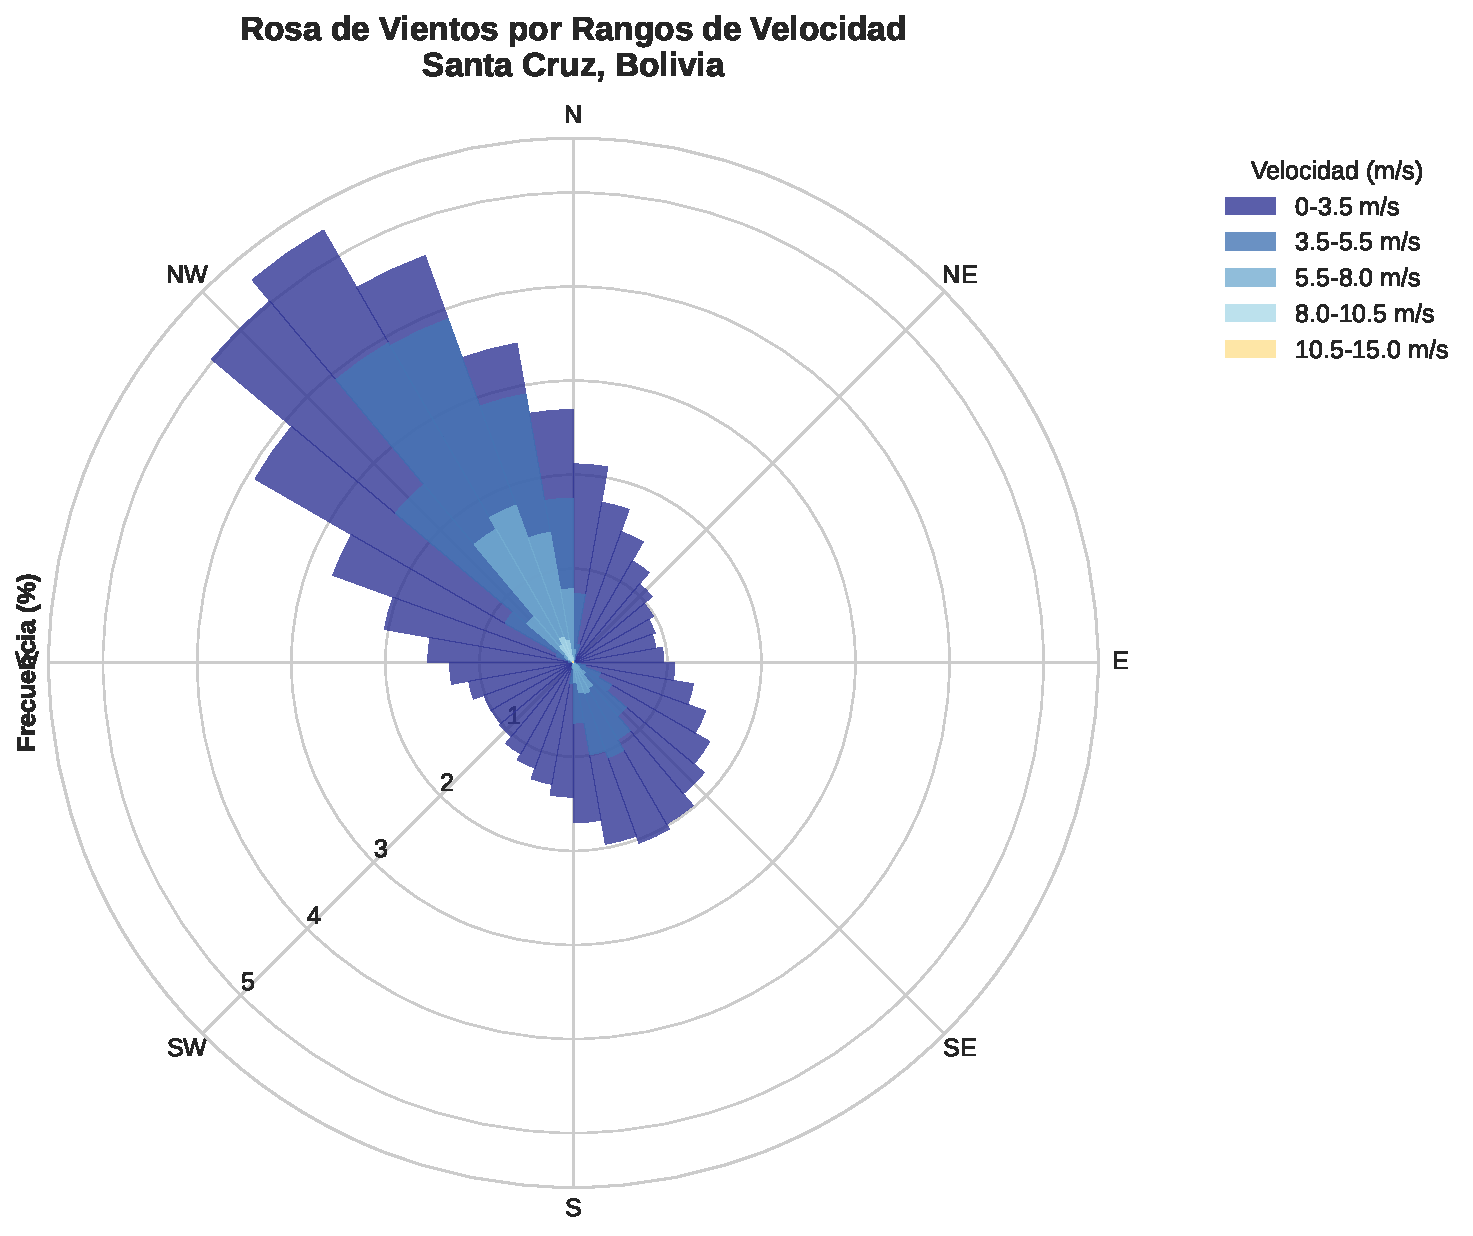
\includegraphics[width=0.6\textwidth]{rosa_vientos_colorizada.pdf}
		\caption{Rosa de los vientos segmentada por intervalos de velocidad.}
		\label{fig:rosa}
	\end{figure}
	
	\subsection{Estimación del Potencial Energético}
	Aplicando el modelo de potencia de la Ec.~\eqref{eq:potencia} con $\rho=1.225\ \mathrm{kg/m^3}$, $D=100\ \mathrm{m}$ y $C_p=0.59$, se obtuvo:
	
	\begin{itemize}
		\item Potencia media generada: $P_\text{media}\approx145\ \mathrm{kW}$
		\item Factor de capacidad: $\mathrm{FC}\approx3.0\%$
		\item Energía anual estimada: $E \approx 1.27\ \mathrm{GWh}\,\text{/año}$
	\end{itemize}
	
	\begin{figure}[H]
		\centering
		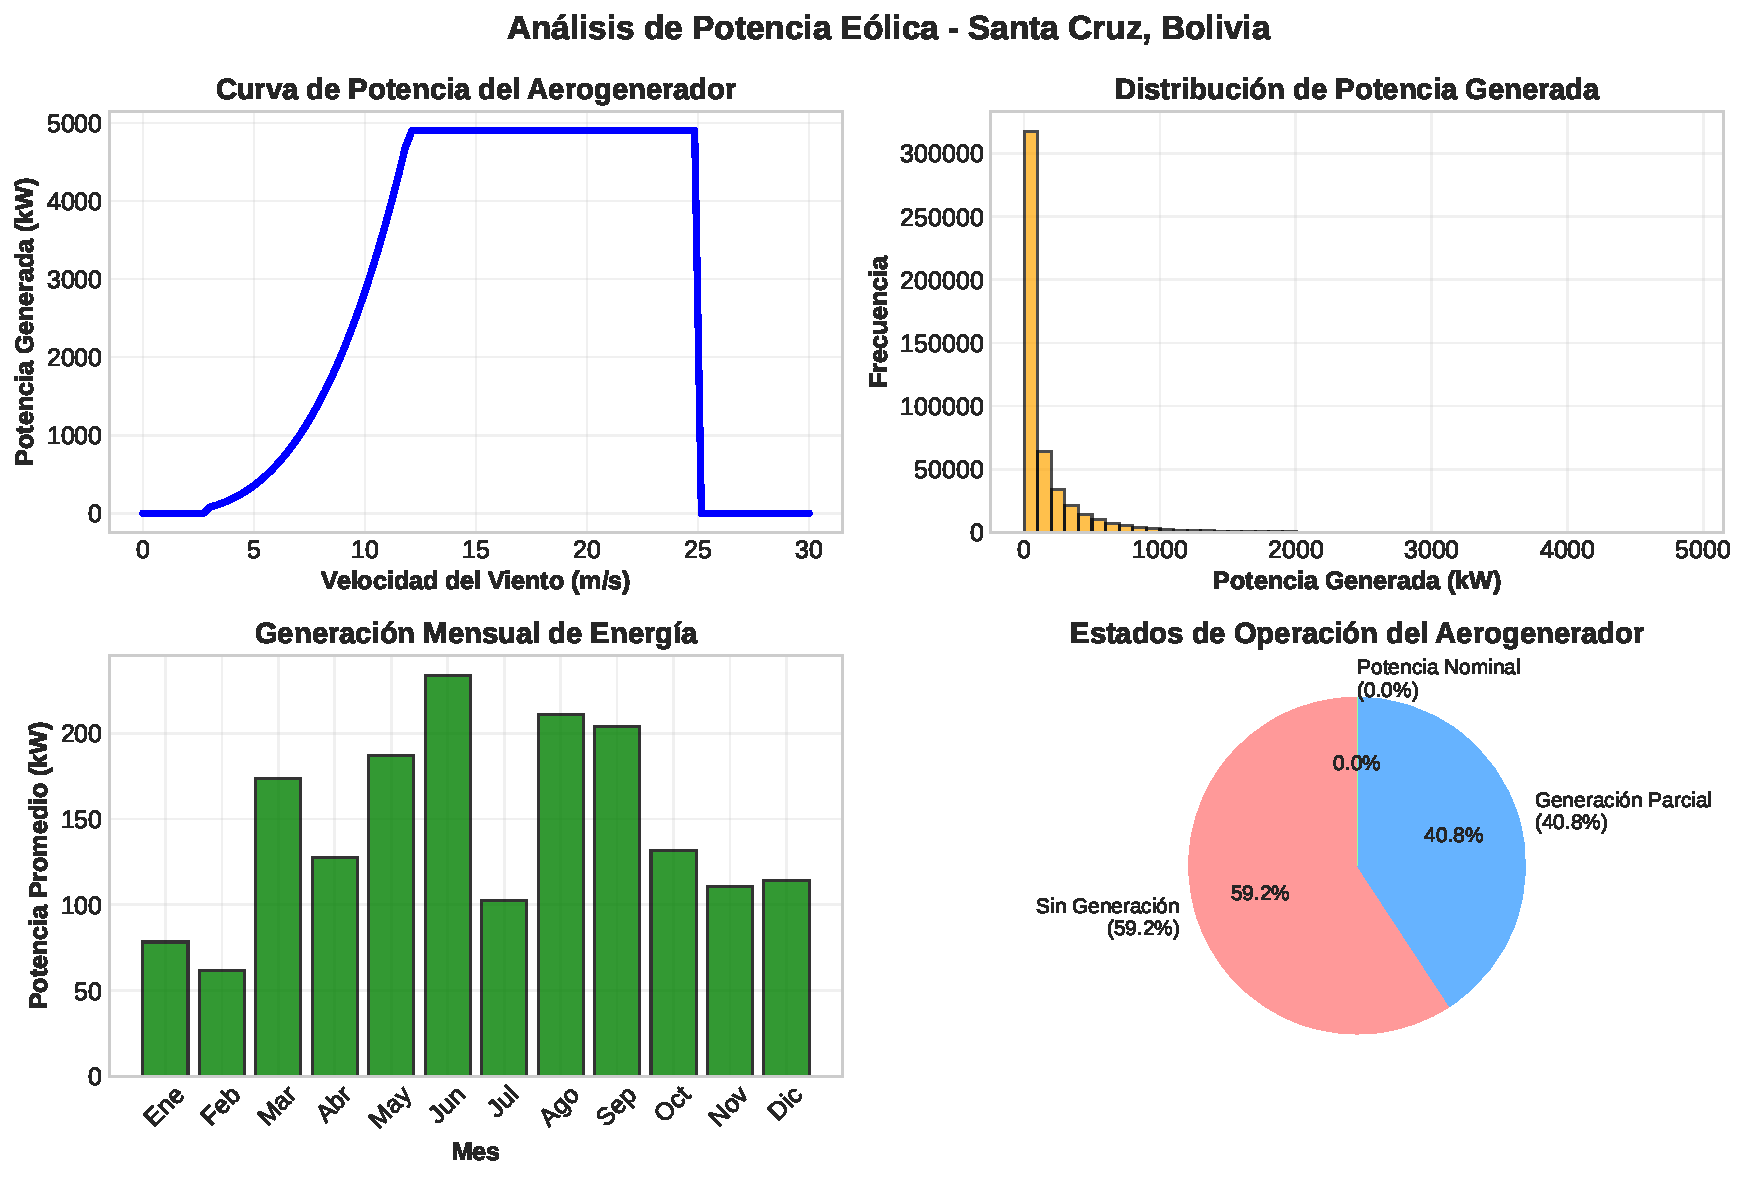
\includegraphics[width=0.8\textwidth]{analisis_potencia.pdf}
		\caption{Perfil de potencia generada y modelo de curva de potencia.}
		\label{fig:potencia}
	\end{figure}
	
	\subsection{Mapa de Velocidad Media}
	El mapa de velocidad media anual (Figura~\ref{fig:mapa}) muestra un ligero gradiente orográfico: las zonas elevadas al este superan apenas los 3.5\,m/s, mientras que la llanura central no alcanza los 3.0\,m/s.
	
	\begin{figure}[H]
		\centering
		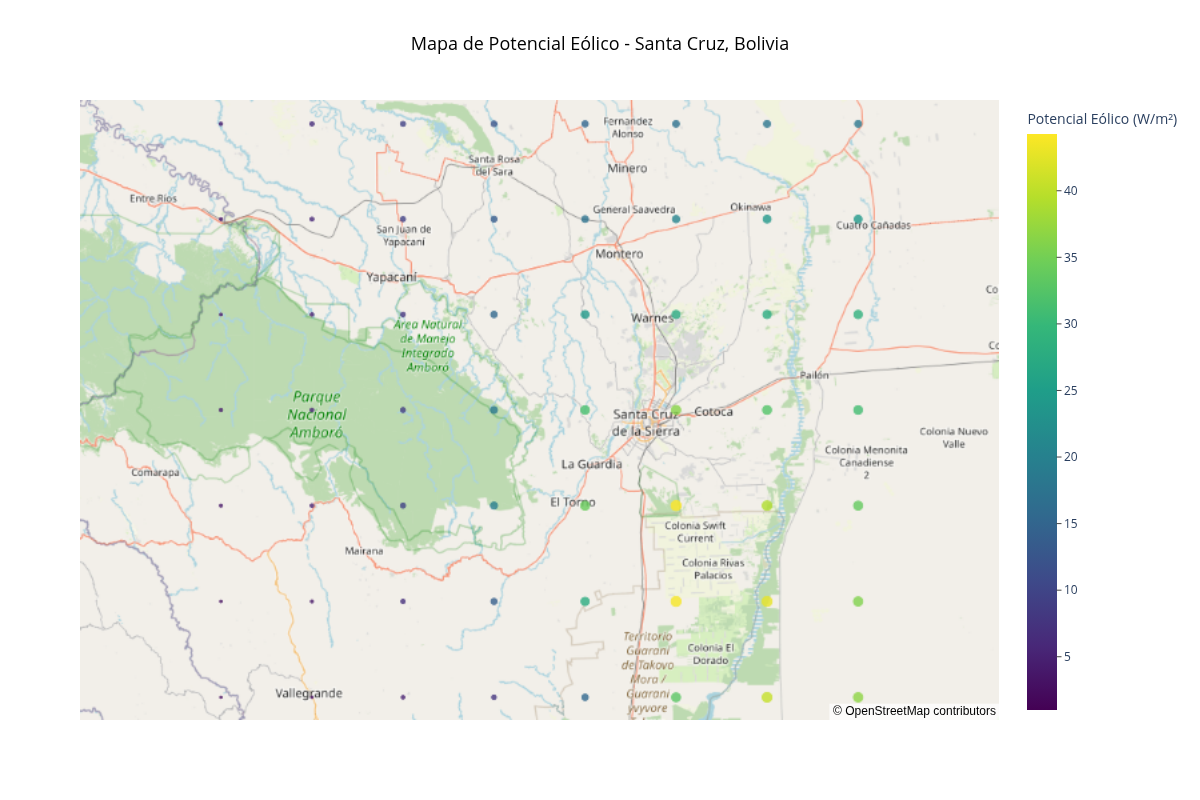
\includegraphics[width=1.0\textwidth]{mapa_velocidades.png}
		\caption{Velocidad media anual del viento en Santa Cruz (ERA5 2024)}
		\label{fig:mapa}
	\end{figure}
	
	\subsection{Discusión de Viabilidad}
	Las velocidades medias anuales cercanas a 2.9\,m/s se encuentran por debajo del umbral rentable típico (>4\,m/s) para parques eólicos comerciales, resultando en factores de capacidad inferiores al 10\%. 
	
	Se recomienda:
	\begin{itemize}
		\item Instalar anemómetros locales para validar el recurso con mayor detalle espacial.
		\item Evaluar turbinas de baja velocidad de arranque para aplicaciones en microredes rurales.
		\item Complementar con energía solar (dada la alta irradiación local) y sistemas de almacenamiento para mitigar la intermitencia.
		\item Ubicar proyectos en las zonas elevadas del este, donde el viento es ligeramente superior.
	\end{itemize}
	
	En resumen, aunque el recurso eólico en Santa Cruz no es alto, presenta potencial para aplicaciones de pequeña escala o proyectos híbridos con otras fuentes renovables.
	
		
	\section{Conclusiones}
		\section{Conclusiones}
		
		A lo largo de este trabajo se realizó un análisis técnico del recurso eólico en el departamento de Santa Cruz, Bolivia, utilizando datos del reanálisis ERA5 correspondientes al año 2024. Se emplearon herramientas computacionales en Python para procesar, visualizar y evaluar estadísticamente las velocidades del viento.
		
		Los resultados muestran que la velocidad media anual del viento en la región es de aproximadamente 2.91 m/s, con una distribución ajustada a una Weibull con parámetros \(c = 3.15\) y \(k = 1.75\). Estas características ubican al recurso eólico de Santa Cruz dentro de una categoría baja, con un potencial energético limitado.
		
		El estudio permitió aplicar técnicas de análisis de datos y modelado estadístico, incluyendo el ajuste de distribuciones, generación de mapas, rosas de viento y estimaciones de potencia, consolidando así una metodología reproducible para la evaluación de recursos renovables.
		
		En conclusión, aunque el recurso eólico en Santa Cruz no presenta condiciones óptimas para generación a gran escala, el presente trabajo cumple con el objetivo de demostrar y aplicar herramientas técnicas para su caracterización mediante datos abiertos y programación científica.
		
	\appendix
	
\end{document}
